\documentclass{article}
\usepackage[ipa]{luatexja-preset}
\usepackage{amssymb,amsfonts}
\usepackage{graphicx}
\usepackage{tikz}
\usepackage{bm}
\usetikzlibrary{intersections,calc,arrows.meta,decorations.pathreplacing}
\title{数学図案集}
\author{加藤公一 Kimikazu KATO}

\begin{document}
\maketitle
\section{三角関数}
\begin{figure}\caption{$\sin$と$\cos$の定義(その1)}
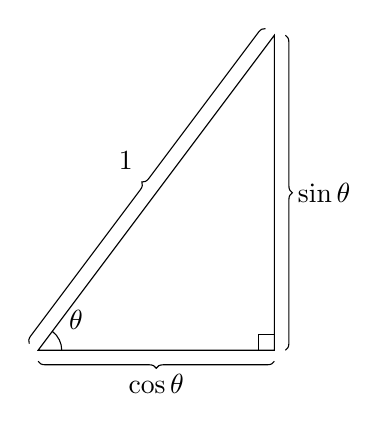
\begin{tikzpicture}
  \coordinate(A) at (0,0);
  \coordinate(B) at (3,0);
  \coordinate(C) at (3,4);
  \coordinate(P) at ($(B)+(-0.2,0.2)$);
  \draw(A)--(B)node[midway,below=5pt]{$\cos\theta$}
  --(C)node[midway,right=5pt]{$\sin\theta$}--cycle node[midway, above left=5pt]{1};
  \draw(P)--($(A)!(P)!(B)$);
  \draw(P)--($(B)!(P)!(C)$);
  \draw(0.3,0)arc(0:{atan(4/3)}:0.3)node[midway, above right]{$\theta$};
  \draw[decorate, decoration={brace, mirror, raise=4pt}](A)--(B);
  \draw[decorate, decoration={brace, mirror, raise=4pt}](B)--(C);
  \draw[decorate, decoration={brace, mirror, raise=4pt}](C)--(A);
\end{tikzpicture}
\end{figure}
\begin{figure}\caption{$\sin$と$\cos$の定義(その2)}
\begin{tikzpicture}
  \def\a{55}
  \draw(0,0) circle(2);
  \draw(0,0)-- ++(\a:2)node[right]{$(\cos\theta,\sin\theta)$};
  \draw[->](-3,0)--(3,0)node[right]{$x$};
  \draw[-Stealth](0,-3)--(0,3)node[above]{$y$};
  \draw(0,0)node[below left]{0};
  \draw(0.3,0)arc(0:\a:0.3)node[midway, above right=0mm]{$\theta$};
  \fill(\a:2)circle(2pt);
  \draw(2,0)node[below right]{$1$};
\end{tikzpicture}
\end{figure}
\begin{figure}\caption{正弦定理}
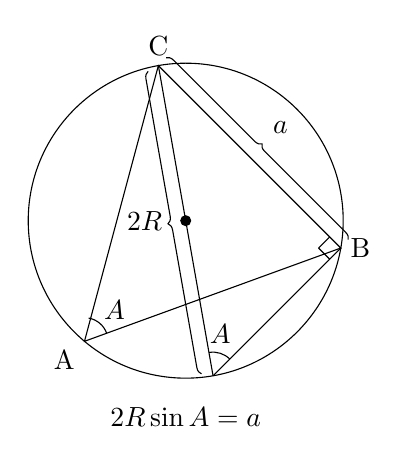
\begin{tikzpicture}
  \def\a{-130}
  \def\b{-10}
  \def\c{100}
  \def\d{\c-180}
  \draw(0,0) circle(2);
  \coordinate(A) at (\a:2);
  \coordinate(B) at (\b:2);
  \coordinate(C) at (\c:2);
  \coordinate(D) at (\d:2);
  \coordinate(P) at ($(B)!0.2cm!(C)!0.2cm!90:(C)$);
  \draw(A)node[below left]{A}--(B)node[right]{B}
  --(C)node[midway, above right=5pt]{$a$}node[above]{C}
  --cycle;
  \draw(C)--(D)node[midway, left=5pt]{$2R$};
  \draw(B)--(D);
  \draw[decorate,
  decoration={brace, mirror, raise=4pt,
    pre=moveto, pre length=0.05cm,
    post=moveto, post length=0.05cm}](C)--(D);
  \draw[decorate, decoration={brace, raise=4pt}](C)--(B);
  \draw(P)--($(C)!(P)!(B)$);
  \draw(P)--($(D)!(P)!(B)$);
  \draw($(D)+({0.3*cos(45)},{0.3*sin(45)})$)arc(45:100:0.3)
  node[midway, above]{$A$};
  \draw($(A)+({0.3*cos(20)},{0.3*sin(20)})$)arc(20:80:0.3);
  \node at ($(A)+({0.3*cos(20)},{0.3*sin(20)})+(0.1,0.3)$) {$A$};
  \fill(0,0)circle(2pt);
  \draw(0,-2.5)node{$2R\sin A=a$};
\end{tikzpicture}
\end{figure}
\begin{figure}\caption{余弦定理}
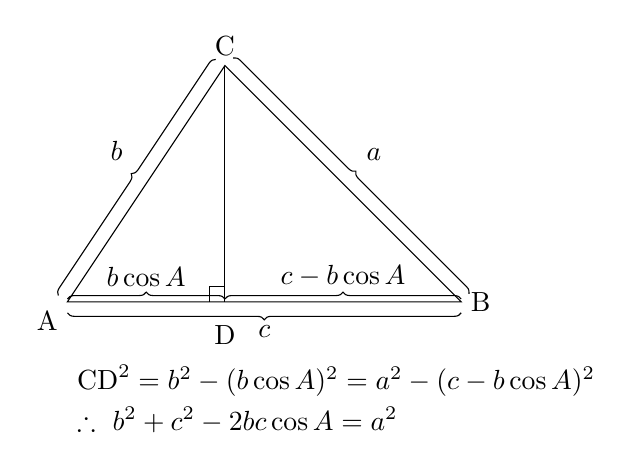
\begin{tikzpicture}
  \coordinate(A) at (0,0);
  \coordinate(B) at (5,0);
  \coordinate(C) at (2,3);
  \coordinate(D) at ($(A)!(C)!(B)$);
  \coordinate(P) at ($(D)+(-0.2,0.2)$);
  \draw(A)node[below left]{A}
  --(B)node[right]{B} node[midway,below=5pt]{$c$}
  --(C)node[above]{C} node[midway,above right=5pt]{$a$}
  --cycle node[midway,above left=5pt]{$b$};
  \draw(C)--(D)node[below=5pt]{D};
  \draw(P)--($(A)!(P)!(D)$);
  \draw(P)--($(C)!(P)!(D)$);
  \draw[decorate, decoration={brace, mirror, raise=4pt}](A)--(B);
  \draw[decorate, decoration={brace, mirror, raise=4pt}](B)--(C);
  \draw[decorate, decoration={brace, mirror, raise=4pt}](C)--(A);
  \draw[decorate, decoration={brace, raise=1pt}](A)--(D);
  \draw[decorate, decoration={brace, raise=1pt}](D)--(B);
  \node at ($(A)!0.5!(D)$) [above=2pt]{$b\cos A$};
  \node at ($(D)!0.5!(B)$) [above=2pt]{$c-b\cos A$};
  \node at (0,-1) [right] {$\mathrm{CD}^2=b^2-(b\cos A)^2=a^2-(c-b\cos A)^2$};
  \node at (0,-1.5) [right] {$\therefore\ b^2+c^2-2bc\cos A=a^2$};
\end{tikzpicture}
\end{figure}
\end{document}
